%!TEX TS-program = xelatex
%!TEX encoding = UTF-8 Unicode

\documentclass[11pt]{extarticle}
% extarticle is like article but can handle 8pt, 9pt, 10pt, 11pt, 12pt, 14pt, 17pt, and 20pt text

\def \ititle {Which Joint Actions Ground Social Cognition}
\def \isubtitle {}
\def \iauthor {Stephen A. Butterfill}
\def \iemail{s.butterfill@warwick.ac.uk}
\date{}


\input{$HOME/Documents/submissions/preamble_steve_handout}

\bibpunct{}{}{,}{s}{}{,}  %use superscript TICS style bib
%remove hanging indent for TICS style bib
%TODO doesnt work
\setlength{\bibhang}{0em}
%\setlength{\bibsep}{0.5em}


%itemize bullet should be dash
\renewcommand{\labelitemi}{$-$}

\begin{document}

\begin{multicols}{3}

\setlength\footnotesep{1em}


\bibliographystyle{newapa} %apalike

%\maketitle
%\tableofcontents





\begin{center}
{\Large
\textbf{Which Joint Actions Ground Social Cognition?}
}

Tuebingen, 6 June 2011

%Stephen A. Butterfill

<s.butterfill@warwick.ac.uk>

\end{center}



\

\begin{center}
{\Large
\textbf{The Challenge}
}
\end{center}

Explain the emergence, in evolution or development, of sophisticated forms of social cognition.



\section{Abilities vs.\ cognition}

A \emph{theory of mind ability} is an ability that exists in part because exercising it brings benefits obtaining which depends on exploiting or influencing facts about others’ mental states.  

\emph{Theory of mind cognition} paradigmatically involves ascribing propositional attitudes such as beliefs, desires and intentions to give rationalising causal explanations of action. 


\section{Theory of mind abilities are widespread}
Children in their second year use pointing to provide information to others\citep{Liszkowski:2006ec} in ways that reflect their partners’ ignorance or knowledge;\citep{Liszkowski:2008al} provide more information to ignorant than knowledgeable partners when making requests;\citep{ONeill:1996um}  predict actions of agents with false beliefs about the locations of objects;\citep{Onishi:2005hm,Southgate:2007js} and select different ways of helping others depending on whether their beliefs are true or false.\citep{Buttelmann:2009gy}

Scrub-jays selectively re-cache their food in ways that prevent competitors from knowing its location.\citep{Clayton:2007fh}

Chimpanzees select routes to approach food which conceal them from a competitor’s view,\citep{Hare:2006ih} and retrieve food using strategies that optimise their return given what a dominant competitor has seen.\citep{Hare:2001ph}



\section{Theory of mind cognition is hard}
Conceptually demanding:
\begin{itemize}\itemsep0pt
\item Acquisition takes several years\citep{Wimmer:1983dz,Wellman:2001lz}
\item Tied to the development of executive function\citep{Perner:1999yr,Sabbagh:2006ke} and language\citep{Astington2005ot}
\item Development facilitated by explicit training\citep{Slaughter:1996fv} and siblings\citep{Clements:2000nc,Hughes:2004zj}
\end{itemize}
%
Cognitively demanding: 
\begin{itemize}
\item Requires attention and working memory in fully competent adults\citep{Apperly:2008jv,McKinnon:2007rr}
\end{itemize}


\

\begin{center}
{\Large
\textbf{The Conjecture}
}
\end{center}

The existence of abilities to engage in joint action partially explain how sophisticated forms of social cognition emerge in evolution or development (or both).


`the unique aspects of human cognition ... were driven by, or even constituted by, social co-operation. ...
[R]egular participation in cooperative, cultural interactions during ontogeny leads children to construct uniquely powerful forms of cognitive representation.'
\citep%[pp.\ 1-3]
{Moll:2007gu}



`perception, action, and cognition are grounded in social interaction%
% … functions traditionally considered hallmarks of individual cognition originated through the need to interact with others
'\citep%[p.\ 103]
{Knoblich:2006bn}


\

\begin{center}
{\Large
\textbf{The Question}
}
\end{center}
If The Conjecture is correct, what could joint action be?

\section{The standard view: shared intention}

`I take a collective action to involve a collective intention.'  \citep%[p.\ 5]
{Gilbert:2006wr}

`The sine qua non of collaborative action is a joint goal [shared intention] and a joint commitment’ 
\citep%[p.\ 181]
{tomasello:2008origins}

`the key property of joint action lies in its internal component \ldots \ in the participants’ having a ``collective'' or ``shared'' intention.' \citep%[pp. 444-5]
{alonso_shared_2009}

`Shared intentionality is the foundation upon which joint action is built.' \citep%[p.\ 381]
{Carpenter:2009wq}

`it is precisely the meshing and sharing of psychological states \ldots \ that holds the key to understanding how humans have achieved their sophisticated and numerous forms of joint activity'
\citep%[p.\ 369]
{Call:2009fk}



\section{What is shared intention?}

The functional role of shared intentions is to: 
(i) coordinate activities; (ii) coordinate planning; and (iii) provide a framework to structure bargaining.\citep%[p.\ 99]
{Bratman:1993je}

For you and I to have a shared intention that we J it is sufficient that: `(1)(a) I intend that we J and (b) you intend that we J; (2) I intend that we J in accordance with and because of la, lb, and meshing subplans of la and lb; you intend that we J in accordance with and because of la, lb, and meshing subplans of la and lb; (3) 1 and 2 are common knowledge between us'.\citep%[View 4]
{Bratman:1993je}


`each agent does not just intend that the group perform the […] joint action. Rather, each agent intends as well that the group perform this joint action in accordance with subplans (of the intentions in favor of the joint action) that mesh' \citep%[p.\ 332]
{Bratman:1992mi}

`philosophers ... postulate complex intentional structures that often seem to be beyond human cognitive ability in real-time social interactions.'
\citep%[p.\ 2022]
{Knoblich:2008hy}




\

\begin{center}
  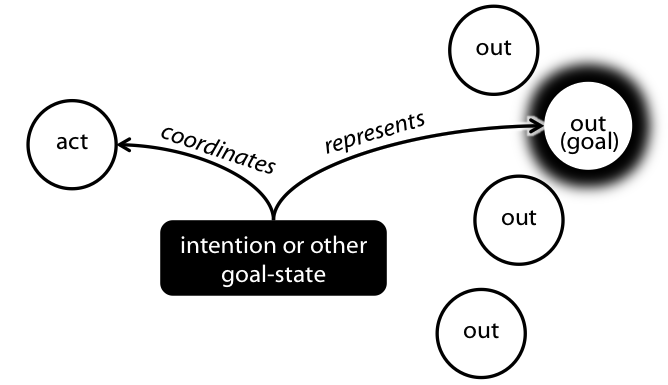
\includegraphics[width=0.3\textwidth]{standard_story.png}
\emph{Figure}: The standard story for individual action.
\end{center}


\section{A joint action is an event with two or more agents\citep{ludwig_collective_2007}}

Given standard claims about action, paradigm cases of joint action do not involve \emph{actions} with two or more agents.

`our primitive actions, the ones we do not by doing something else, ... these are all the actions there are.'\citep%[p.\ 59]
{Davidson:1971fz}

\subsection{Individual event agency}
Two events \emph{overlap} just if a (perhaps improper) part of one is a (perhaps improper) part of the other.

\textbf{singular grounding} 
Event $D$ \emph{grounds} $E$, if: $D$and $E$ occur; 
$D$ is a (perhaps improper) part of $E$; and 
$D$ causes every event that is a proper part of $E$ but does not overlap $D$.

To be the \emph{agent of an event} is to be the agent of the action which grounds it.\citep%[p.\ 81]
{pietroski_actions_1998}


\subsection{Event agency generalised}
Two or more events \emph{overlap} just if any (perhaps improper) part of one of these events is a (perhaps improper) part of any of the other events.

\textbf{plural grounding} 
Events $D_1$, ...\ $D_n$ \emph{ground} $E$, if: $D_1$, ...\ $D_n$ and $E$ occur; 
$D_1$, ...\ $D_n$ are each (perhaps improper) parts of $E$; and 
every event that is a proper part of $E$ but does not overlap  $D_1$, ...\ $D_n$ is caused by some or all of $D_1$, ...\ $D_n$.

For an individual to be \emph{among the agents of an event} is for there to be actions $a_1$, ...\ $a_n$ which ground this event where the individual is an agent of some (one or more) of these actions.


\section{Goal-directed joint action}
A \emph{goal} is an outcome to which actions are, or might be, directed.  A \emph{goal-state} is an intention or other state of an agent linking an action to a goal to which it is directed.

A \emph{goal-directed joint action} is a joint action which, taken as a whole, is directed to a goal.

An outcome is the \emph{teleological function of an action} just if (i) in the past, actions of this type have caused outcomes of this type; (ii) this action happens now in part because (i).\citep{Wright:1976ls}



\textbf{Distributive goal}.  The \emph{distributive goal} of two or more agents' activities is G: each agent's activities are individually directed to G.

\textbf{Collective goal}.  The \emph{collective goal} of a joint action is G:
(a) each agent’s activities are individually directed to G (i.e. G is a distributive goal);
(b) the agents’ activities are coordinated; and 
(c) coordination of this type would normally  facilitate occurrences of outcomes of G's type

\textbf{Shared goal}.  The \emph{shared goal} of two or more agents' activities is G: (a) G is a collective goal of their activities; 
(b) each agent can identify each of the other agents in a way that doesn't depend on knowledge of the goal or	 actions directed to it;
(c) each agent expects each of the other agents to perform activities directed to G; and 
(d) each agent expects G to occur as a common effect of all their goal-directed actions, or to be partly constituted by all of their goal-directed actions.

\ %remove if possible --- formatting weirdness

\ %remove if possible --- formatting weirdness


\footnotesize 
\bibliography{$HOME/endnote/phd_biblio}

\end{multicols}

\end{document}